\chapter{Modelo matemático}
\cleanchapterquote{In mathematics, you don’t understand things. You just get used to them.}{John von Neumann}{(mathematician, physicist, computer scientist, and polymath.)}

En el presente capitulo se aborda el modelo matemático para el seguimiento de objetivos de una gimbal embebida en un UAV.

\section{Marco de referencia}
Los movimientos de la gimbal se basan en las coordenadas horizontales de azimuth y elevación, para gimbal de 3 grados de libertad
se agrega un tercer eje cuyo movimiento se conoce como roll. El eje de azimuth y la elevación se visualizan más fácilmente al 
pensar en la posición de un objeto en relación con el horizonte.
\begin{center}
	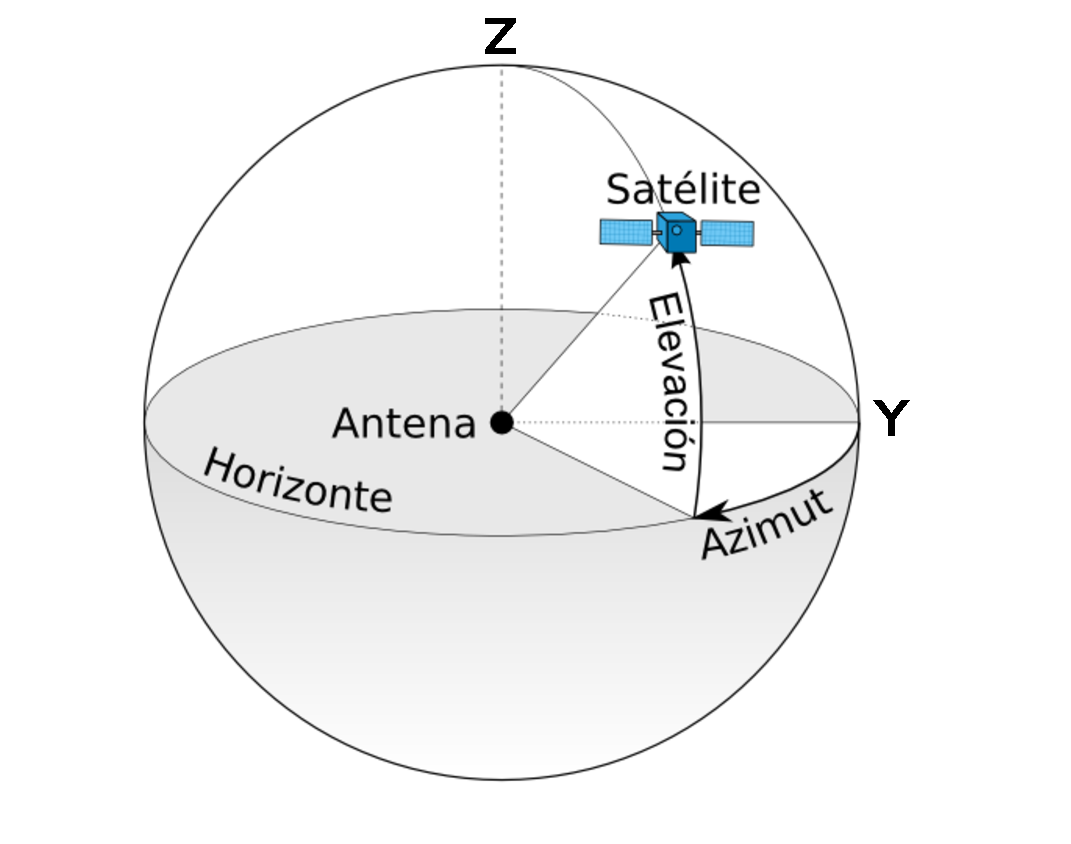
\includegraphics[width=0.55\textwidth]{Contenido/Cuerpo/Capitulo3/Fig1.eps}
	\captionof{figure}{Angulo de azimuth}
	\label{fig:ModeloMat:Fig1}
\end{center}
El angulo de azimuth es la posición alrededor del horizonte, medida desde un punto de referencia como el norte verdadero o el sur 
verdadero. Los movimientos de azimuth ocurren alrededor del eje Z (vertical).

La elevación es la distancia del objeto por encima o por debajo del horizonte (también conocida como altitud en aplicaciones de 
astronomía y aeroespaciales). Los movimientos de elevación ocurren alrededor del eje Y.

Los movimientos de balanceo ocurren alrededor del eje X a medida que gira con los ejes Y y Z.\\
El control que se hace en la gimbal está dado por un motor con control de posición y una IMU (sensor inercial).Dicha gimbal esta
montada en la parte delantera del vehículo aéreo como se muestra en la siguiente figura.
\begin{center}
	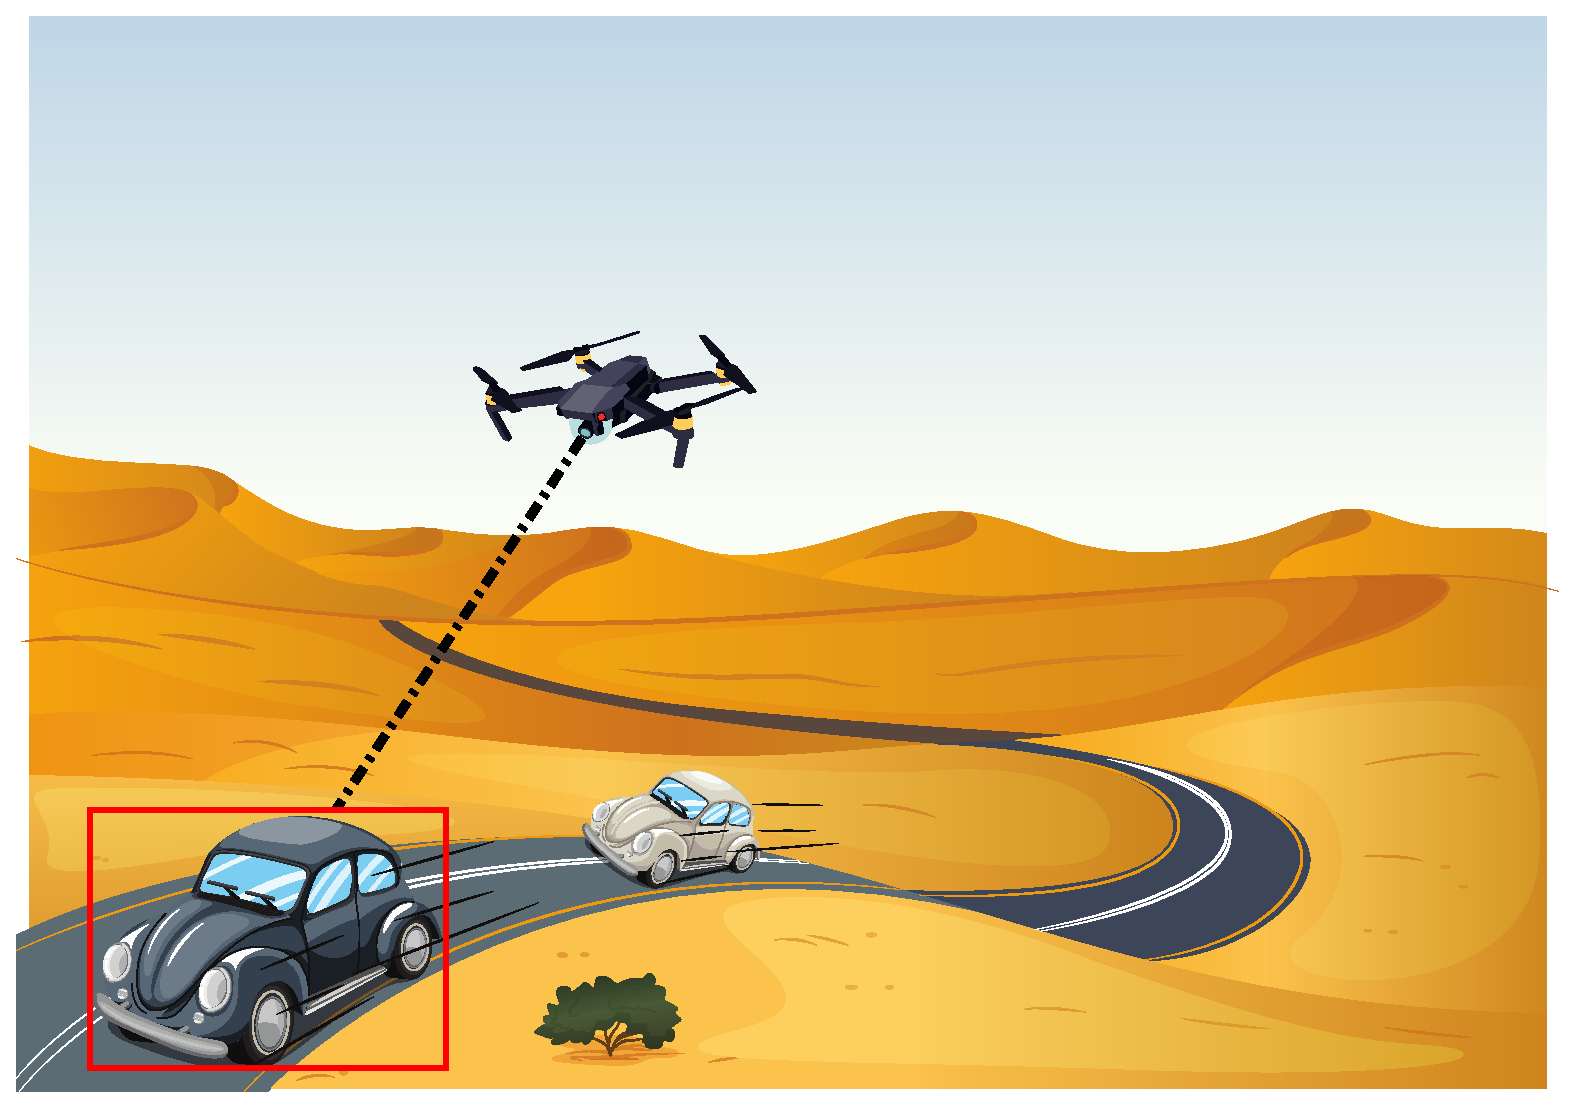
\includegraphics[width=0.55\textwidth]{Contenido/Cuerpo/Capitulo3/Fig2.eps}
	\captionof{figure}{Seguimiento de un objetivo utilizando una cámara sujeta a una gimbal embebida en un vehículo aéreo no tripulado.}
	\label{fig:ModeloMat:Fig1}
\end{center}
